\chapter{Running a Spark Batch Application in Java}
\par In this section, we will create a Spark Batch application in Java (a simple WordCount), load it locally on the node and launch it.
%Intro\footnotemark\\
\begin{spacing}{1.2}
%note en bas de page
\section{Installing Apache Maven}

\par Download and unzip "apache-maven-3.5.0-bin.tar.gz"
\\
\begin{figure}[!htb] 
\begin{center} 
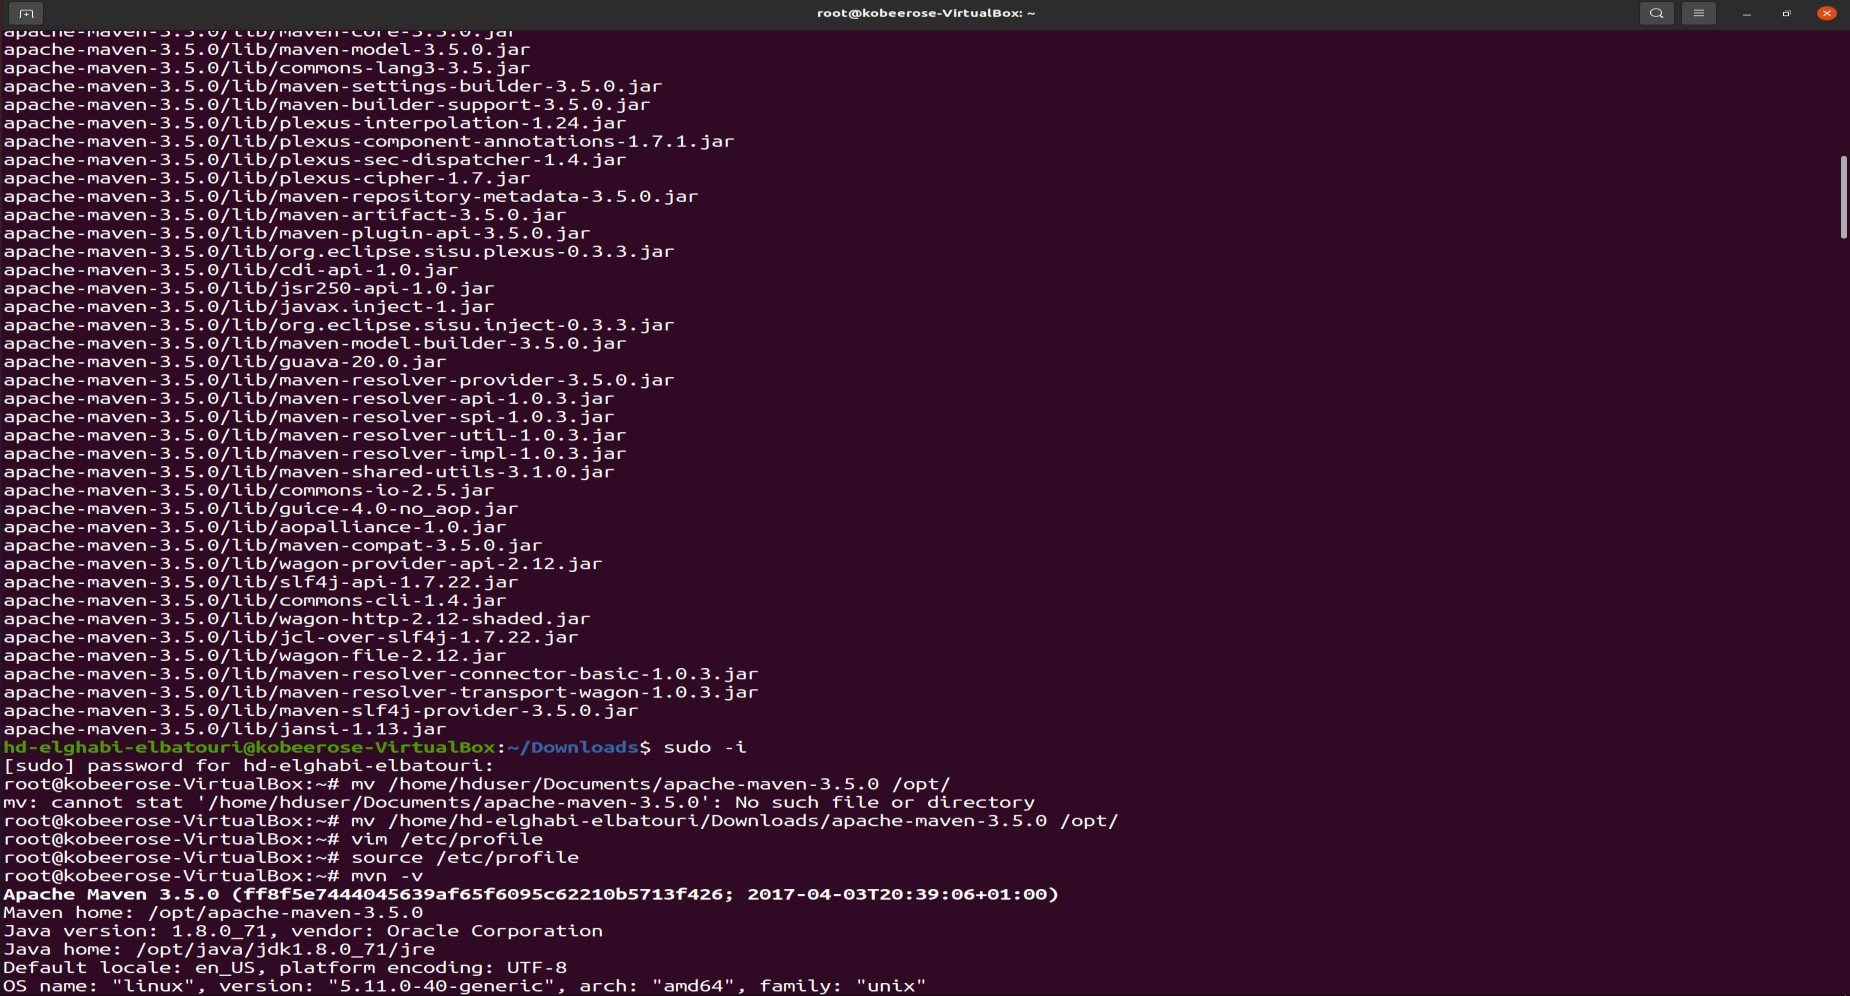
\includegraphics[width=1\linewidth]{Big_Data/Spark/Running a Spark Batch app in Java/Installing Maven} 
\end{center} 
\caption{Installing Maven} 
\end{figure} 
\FloatBarrier



\par Creating a Maven project.
\\
\begin{figure}[!htb] 
\begin{center} 
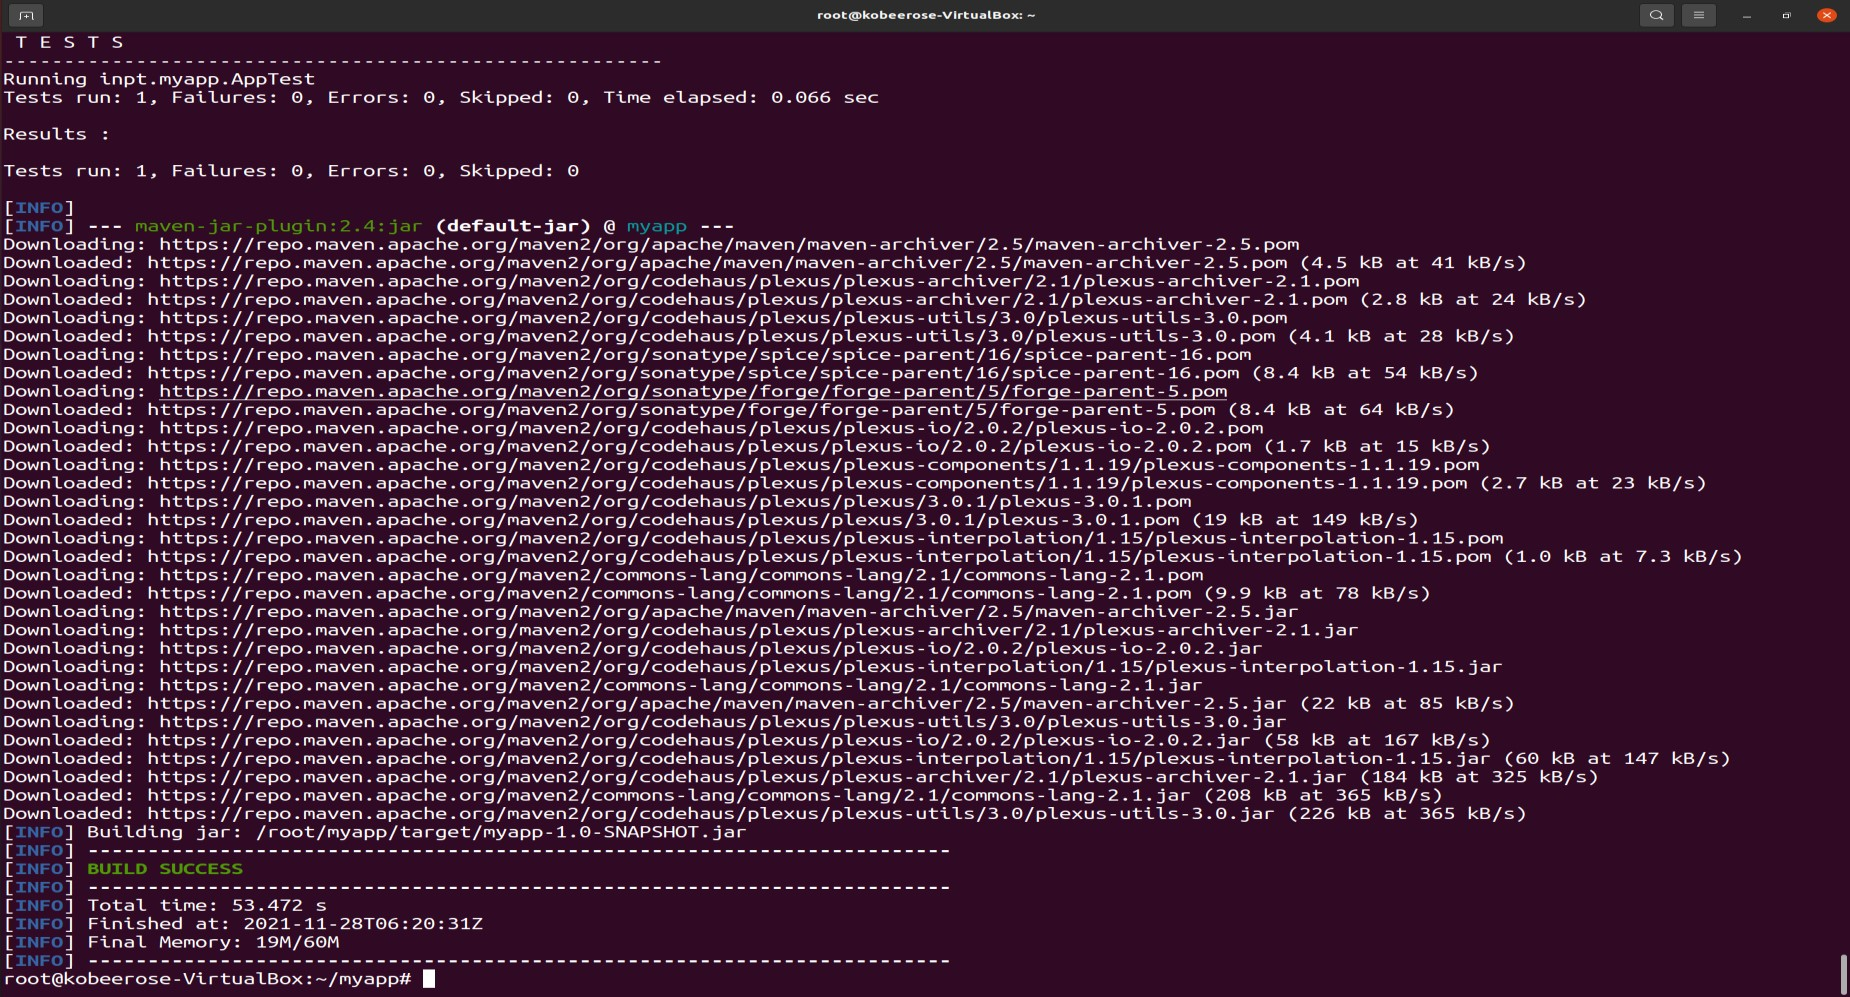
\includegraphics[width=1\linewidth]{Big_Data/Spark/Running a Spark Batch app in Java/Maven Build Success} 
\end{center} 
\caption{Maven Build Success} 
\end{figure} 
\FloatBarrier

\par To see the entire tree structure of the project, we will install the "tree" and view our the project tree:
\\
\begin{figure}[!htb] 
\begin{center} 
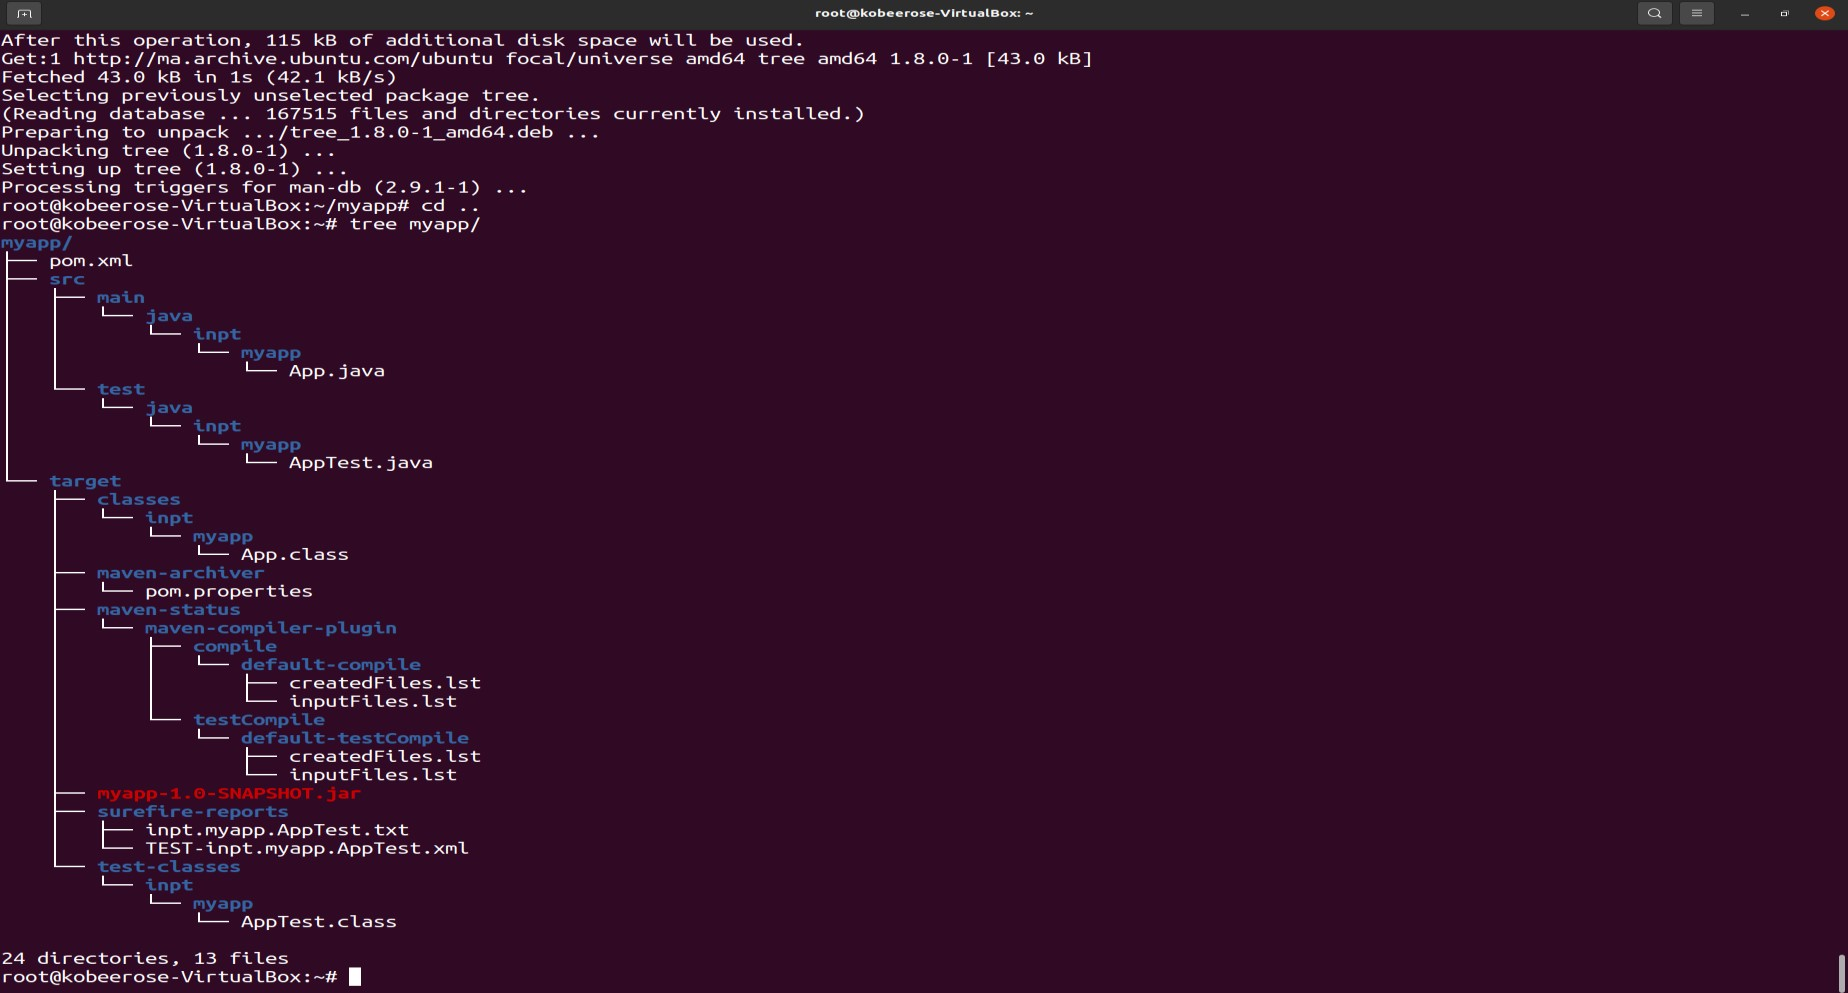
\includegraphics[width=1\linewidth]{Big_Data/Spark/Running a Spark Batch app in Java/App tree} 
\end{center} 
\caption{App tree} 
\end{figure} 
\FloatBarrier

\section{Reconfiguration of the Maven project}

\par we add the necessary dependencies in the "pom.xml" file.
\\
\begin{figure}[!htb] 
\begin{center} 
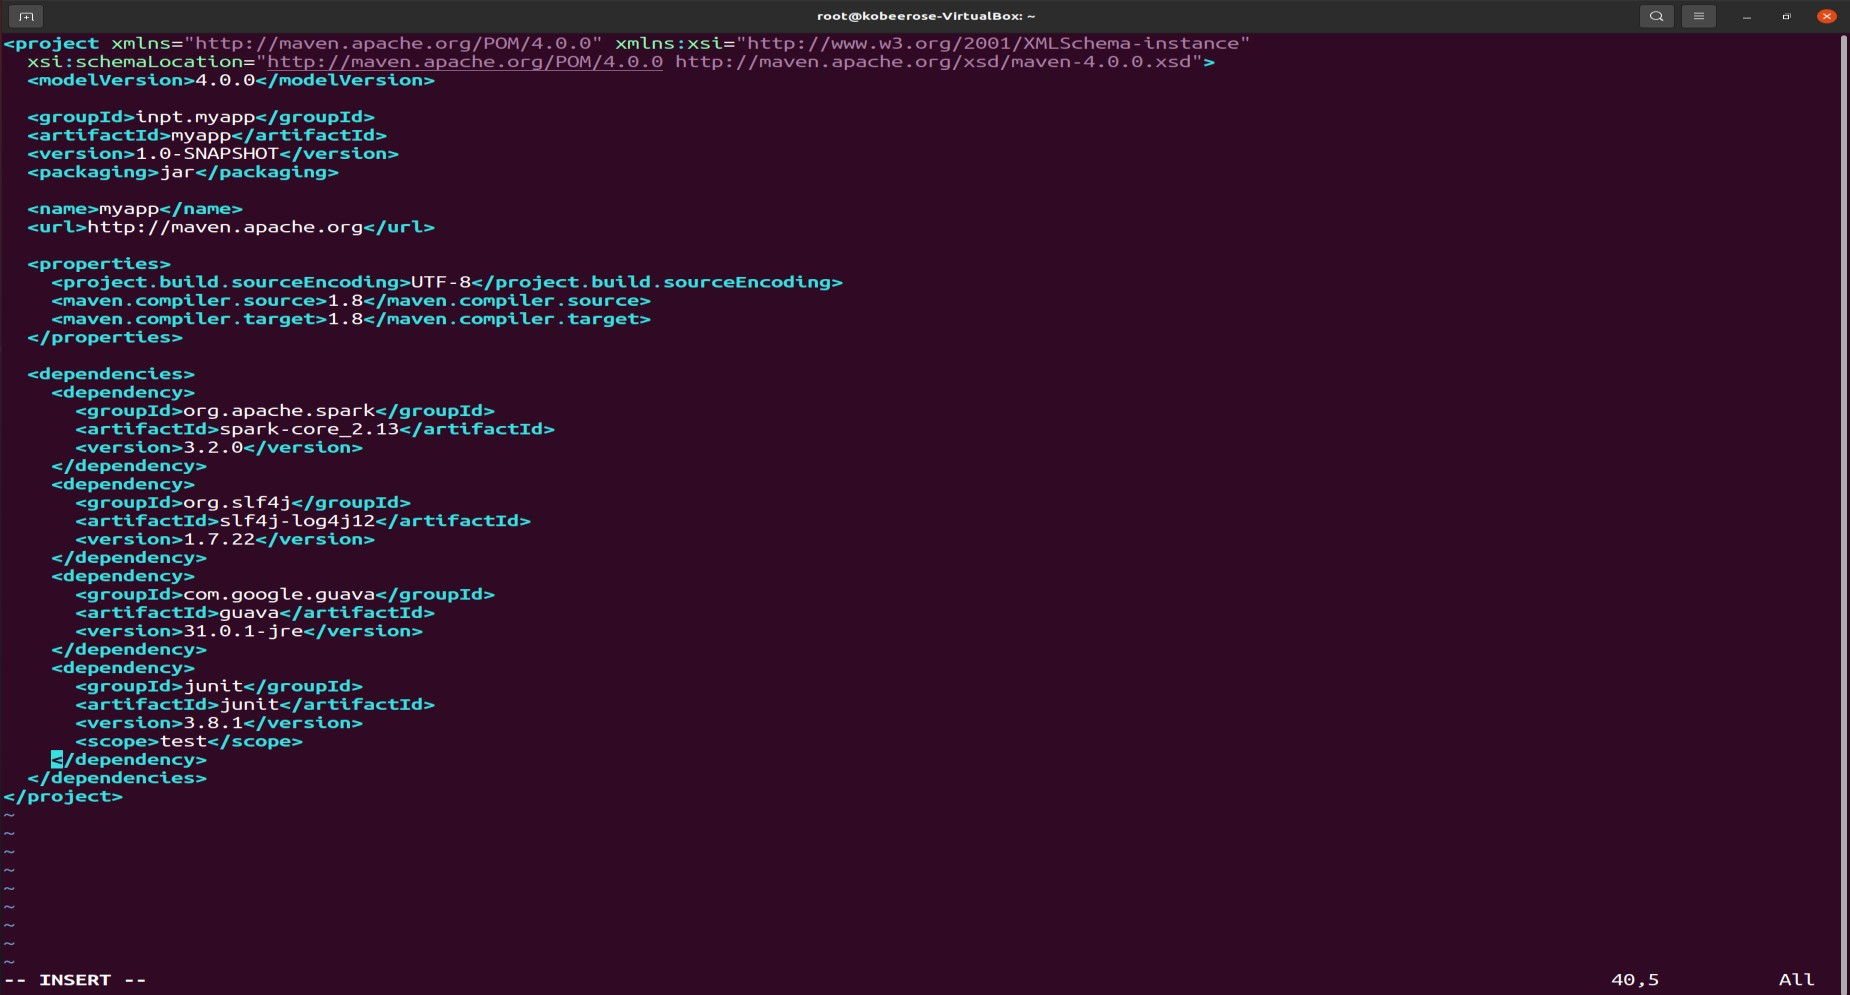
\includegraphics[width=1\linewidth]{Big_Data/Spark/Running a Spark Batch app in Java/pom.xml config} 
\end{center} 
\caption{pom.xml config} 
\end{figure} 
\FloatBarrier



\par Renaming App.java to WordCountTask.java and changing its content to Word Count algorithm.
\\
\begin{figure}[!htb] 
\begin{center} 
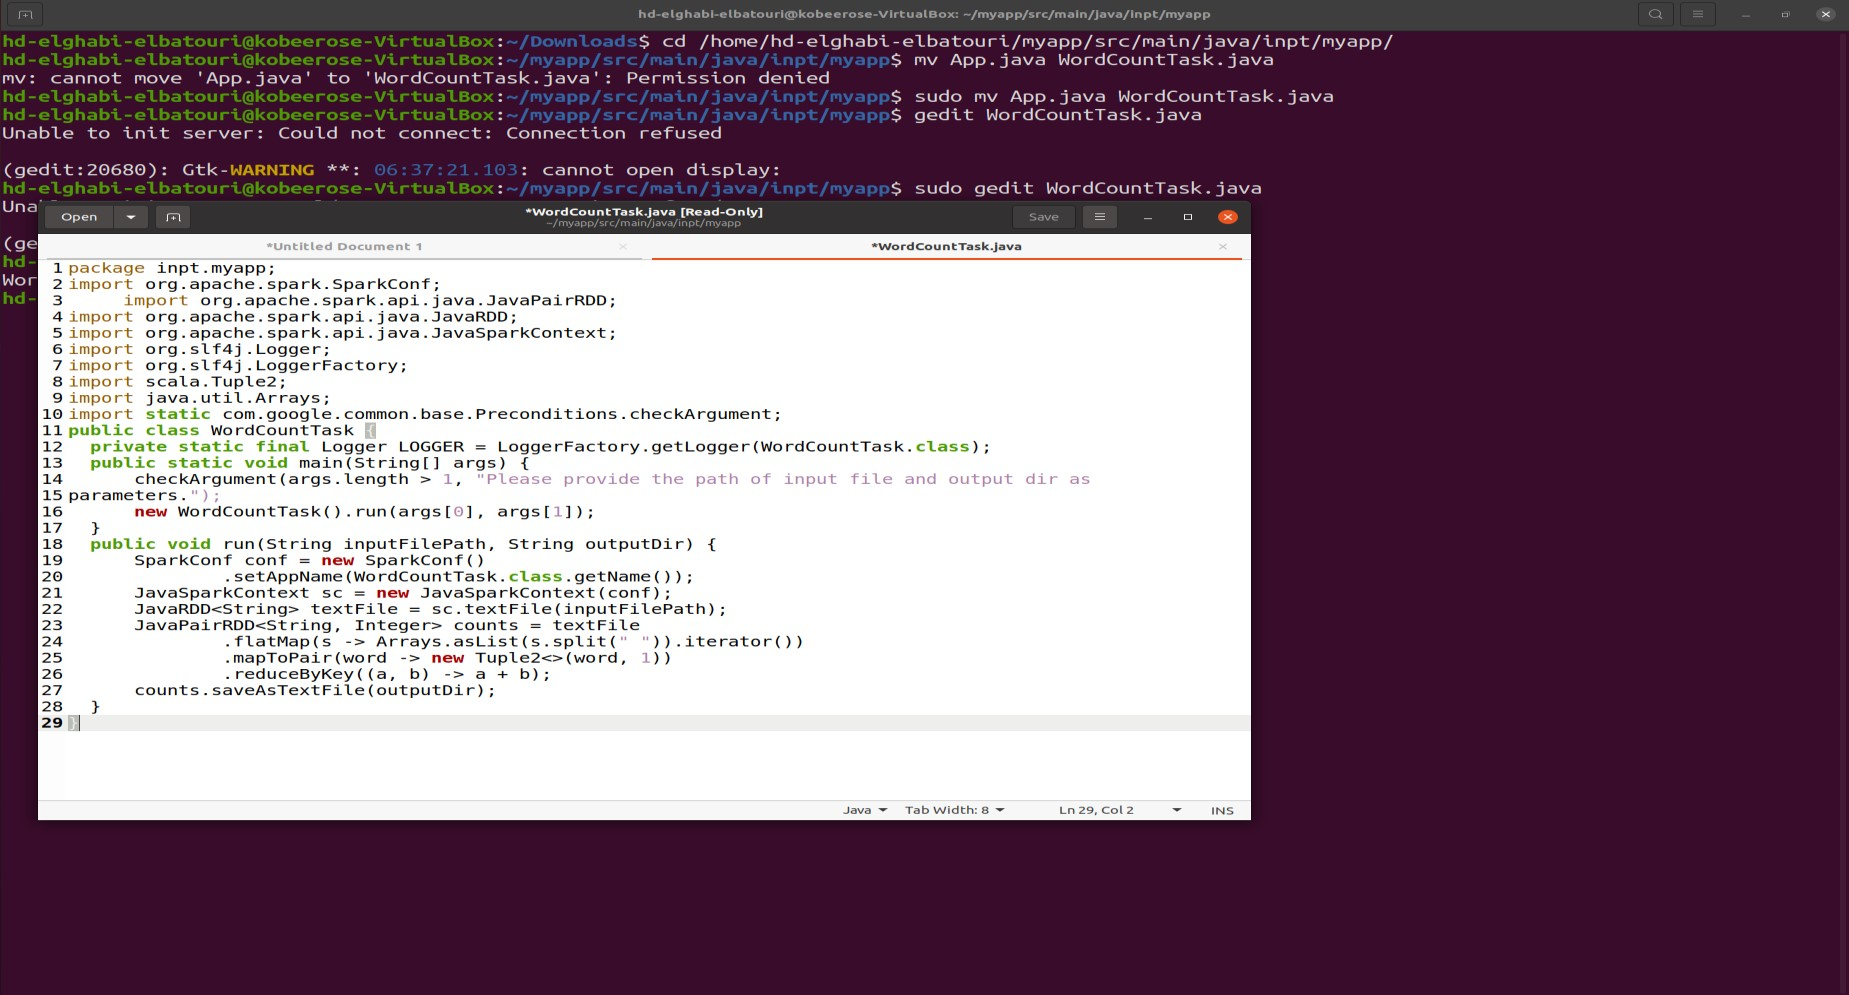
\includegraphics[width=1\linewidth]{Big_Data/Spark/Running a Spark Batch app in Java/WordCountTask.java} 
\end{center} 
\caption{WordCountTask.java} 
\end{figure} 
\FloatBarrier

\par Rebuilding the app with mvn package command.
\\
\begin{figure}[!htb] 
\begin{center} 
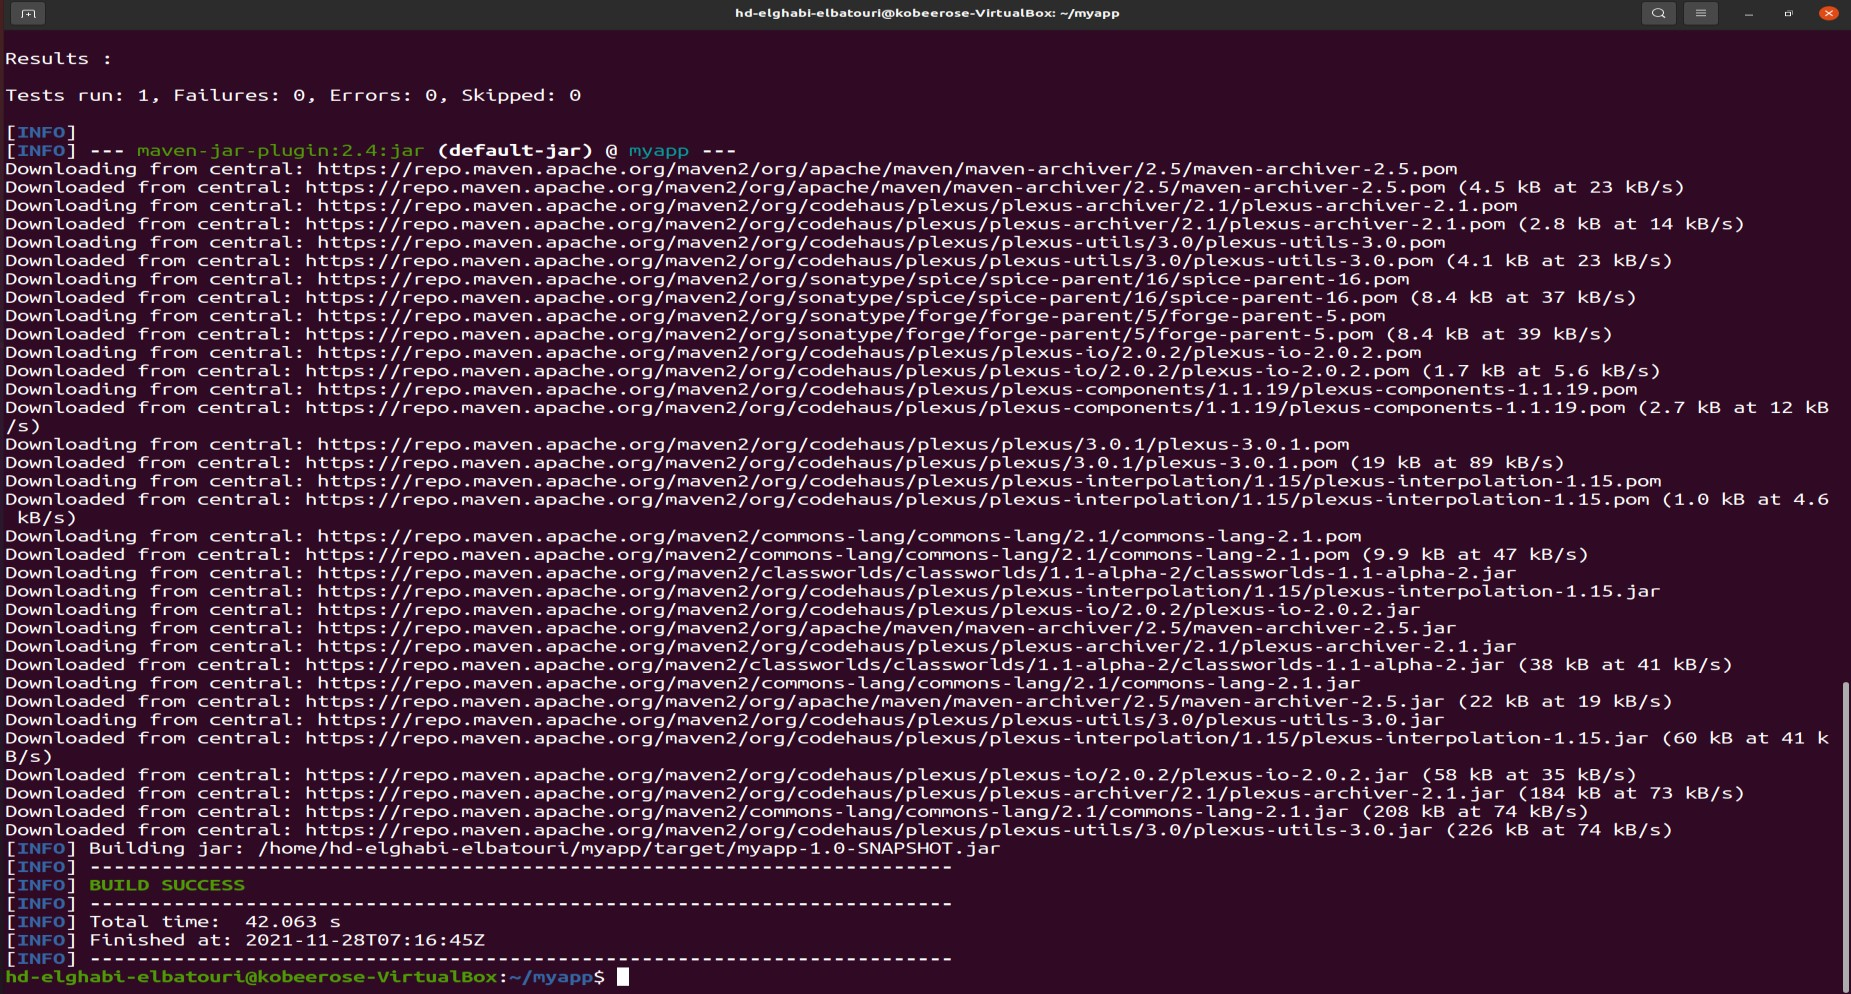
\includegraphics[width=1\linewidth]{Big_Data/Spark/Running a Spark Batch app in Java/Build with WordCount} 
\end{center} 
\caption{Build with WordCount} 
\end{figure} 
\FloatBarrie

\section{Cleaning and formatting the hadoop node}

\par Now, we clean and Format the hadoop nodes Then, we reformatting of the node.
\\
\begin{figure}[!htb] 
\begin{center} 
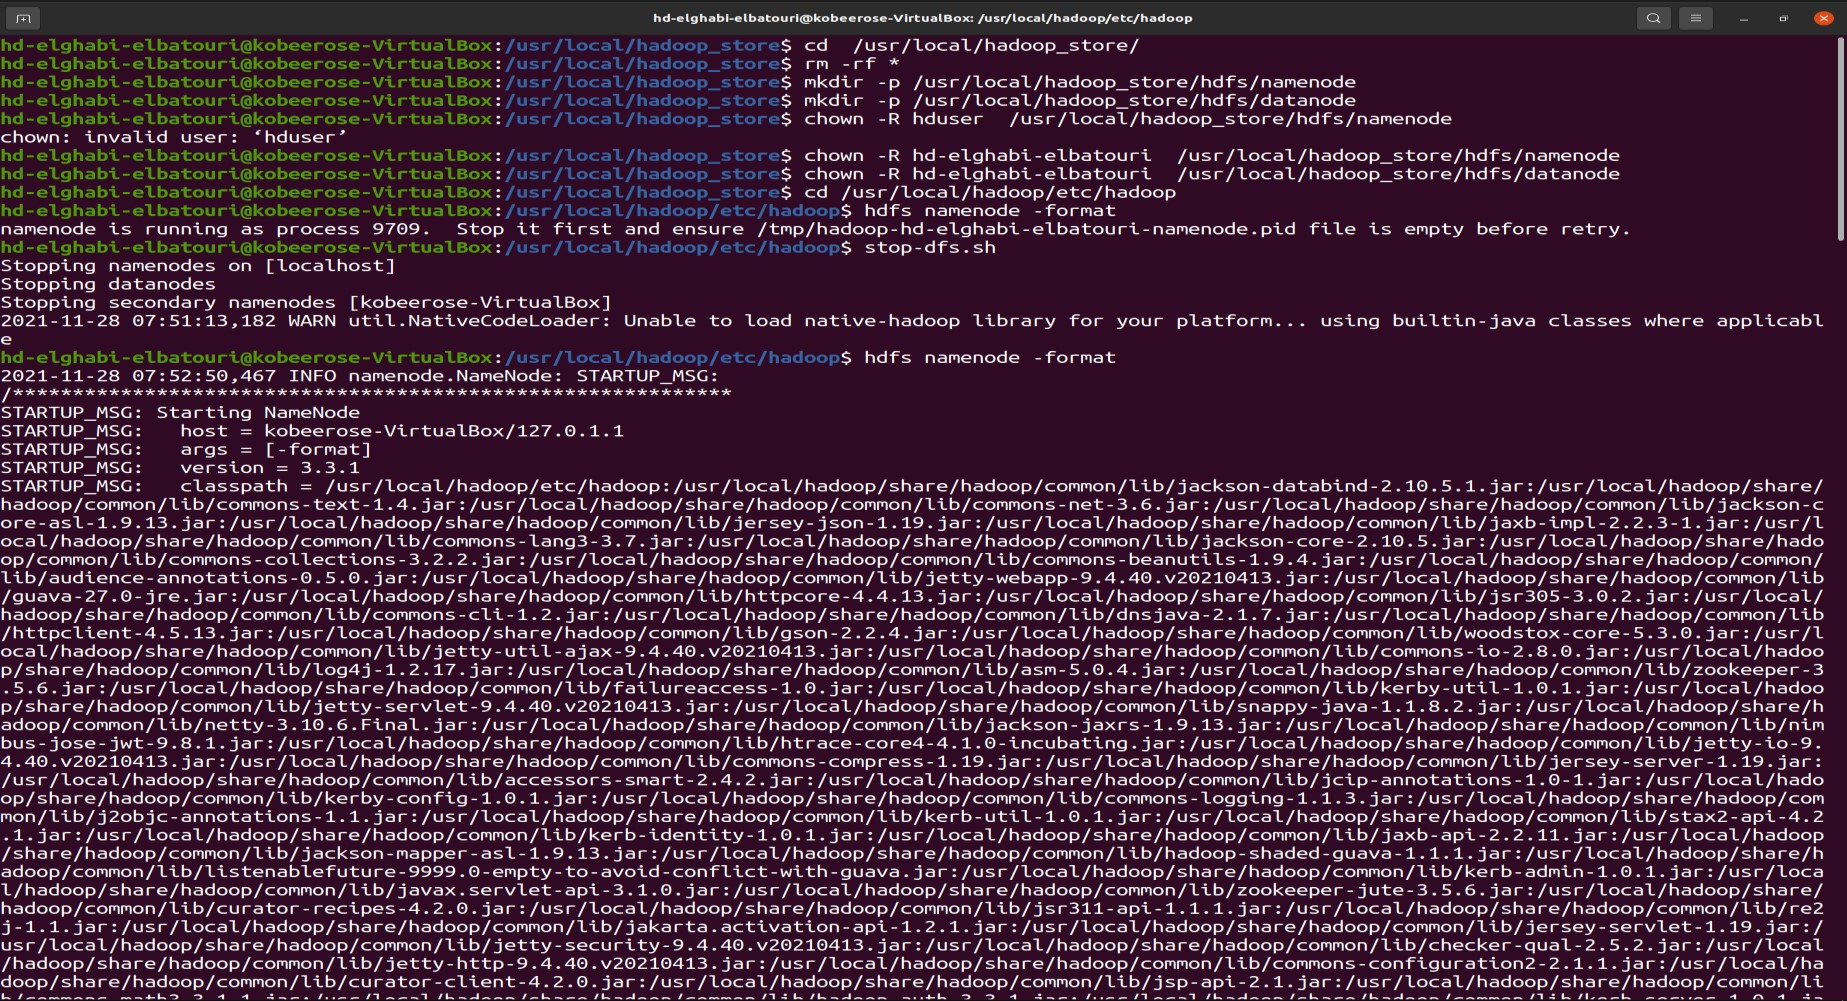
\includegraphics[width=1\linewidth]{Big_Data/Spark/Running a Spark Batch app in Java/Clearning and formatting hadoop nodes} 
\end{center} 
\caption{Clearning and formatting hadoop nodes} 
\end{figure} 
\FloatBarrier



\par Let's check the state of our nodes.
\\
\begin{figure}[!htb] 
\begin{center} 
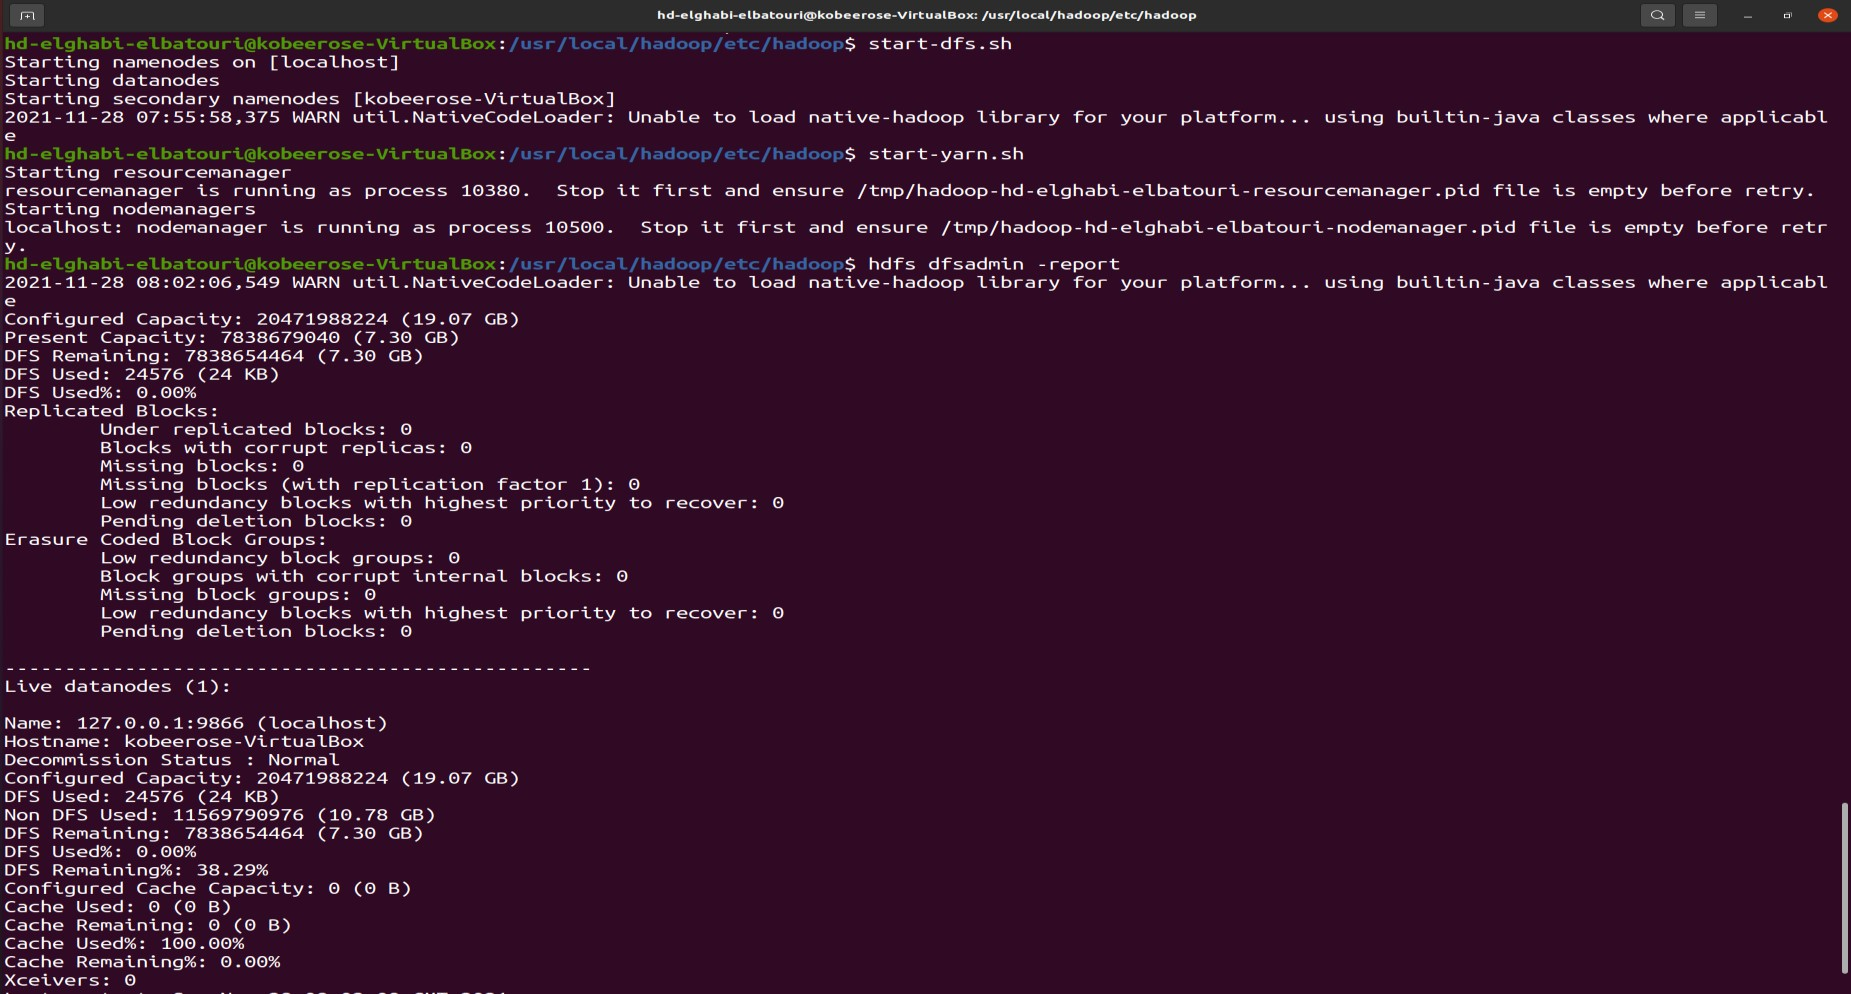
\includegraphics[width=1\linewidth]{Big_Data/Spark/Running a Spark Batch app in Java/Checking live node} 
\end{center} 
\caption{Checking live node} 
\end{figure} 
\FloatBarrier

\section{Putting the poeme.txt file in HDFS}

\par We will put the poeme.txt in the HDFS same as before.
\\
\begin{figure}[!htb] 
\begin{center} 
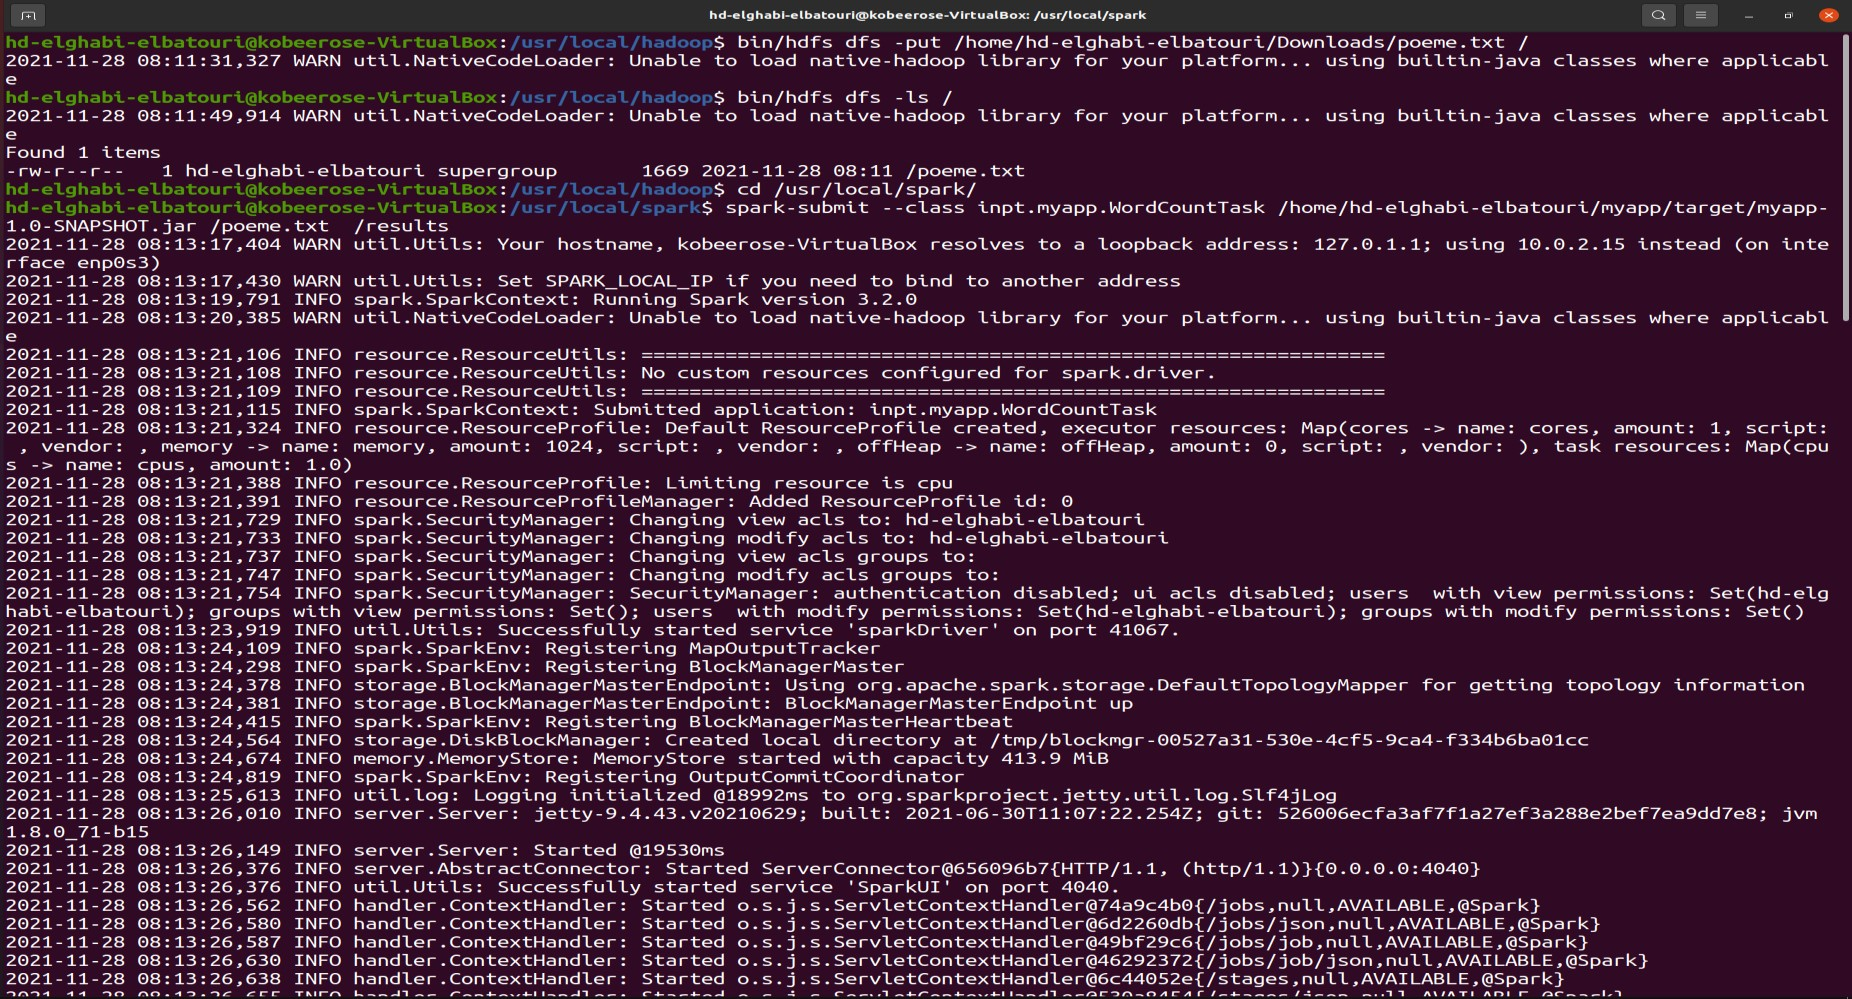
\includegraphics[width=1\linewidth]{Big_Data/Spark/Running a Spark Batch app in Java/Spark Submit} 
\end{center} 
\caption{Spark Submit} 
\end{figure} 
\FloatBarrier
\par And finally we check the final results.
\\
\begin{figure}[!htb] 
\begin{center} 
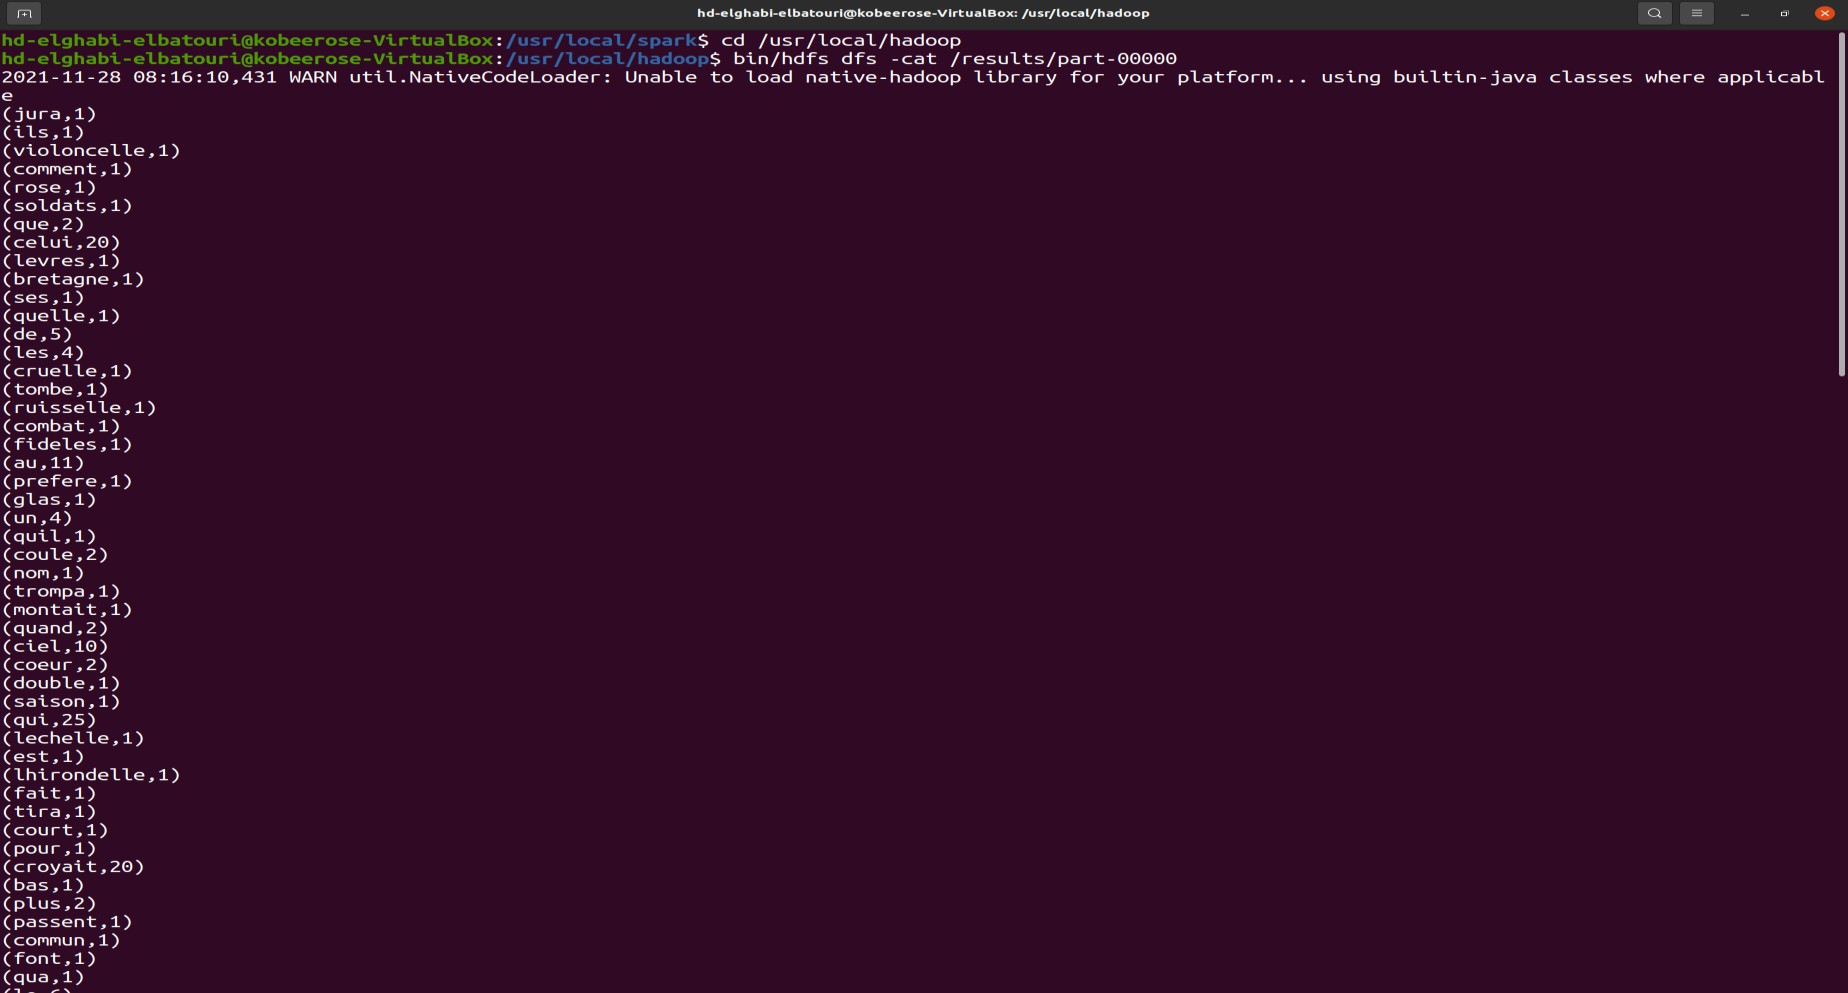
\includegraphics[width=1\linewidth]{Big_Data/Spark/Running a Spark Batch app in Java/Final results} 
\end{center} 
\caption{Final results} 
\end{figure} 
\FloatBarrier



\end{spacing}